\section{Introduction}
\label{sec:introduction}

A display in a shared space can change roles several times a day. It can show the time, count down a scheduled examination, become a stopwatch, and display an important notice when an announcement is needed. In corridors, offices, classrooms, examination halls, and playgrounds, these functions give people a common point of reference. These displays, if connected to a web dashboard, allow the people responsible for the space to change its content and schedule its behavior without physically accessing the device.

Providing that flexibility, however, involves more than simply sending text to a screen. If it's a notice, it can be easily delivered as a remote command. But when it's a scheduled countdown/countup, it must progress locally once its timing information has been received. The device needs to retain enough information to restore its intended behavior after a restart. For example, restarting a display during an examination should not reset the countdown or extend the scheduled interval. Installation and maintenance introduce further requirements: users need a way to configure connectivity, and firmware updates must be possible after the display has been mounted. We address these requirements through an Internet of Things (IoT) system.

We developed a connected time and information display that includes selectable clockfaces, scrolling notices and alerts, a stopwatch, scheduled count-up and countdown features. Users manage the devices through a web dashboard, which communicates with them over Wi-Fi using the Message Queuing Telemetry Transport (MQTT) protocol. Each device executes its display and timing functions locally. The implementation combines an ESP32-S3 controller running Zephyr RTOS with chained HUB12 LED matrix display panels and a custom PCB. Network time synchronization, a real-time clock, persistent settings, Wi-Fi configuration through access point (AP) mode, and over-the-air updates using signed firmware support operation after installation.

\begin{figure}[t]
\centering
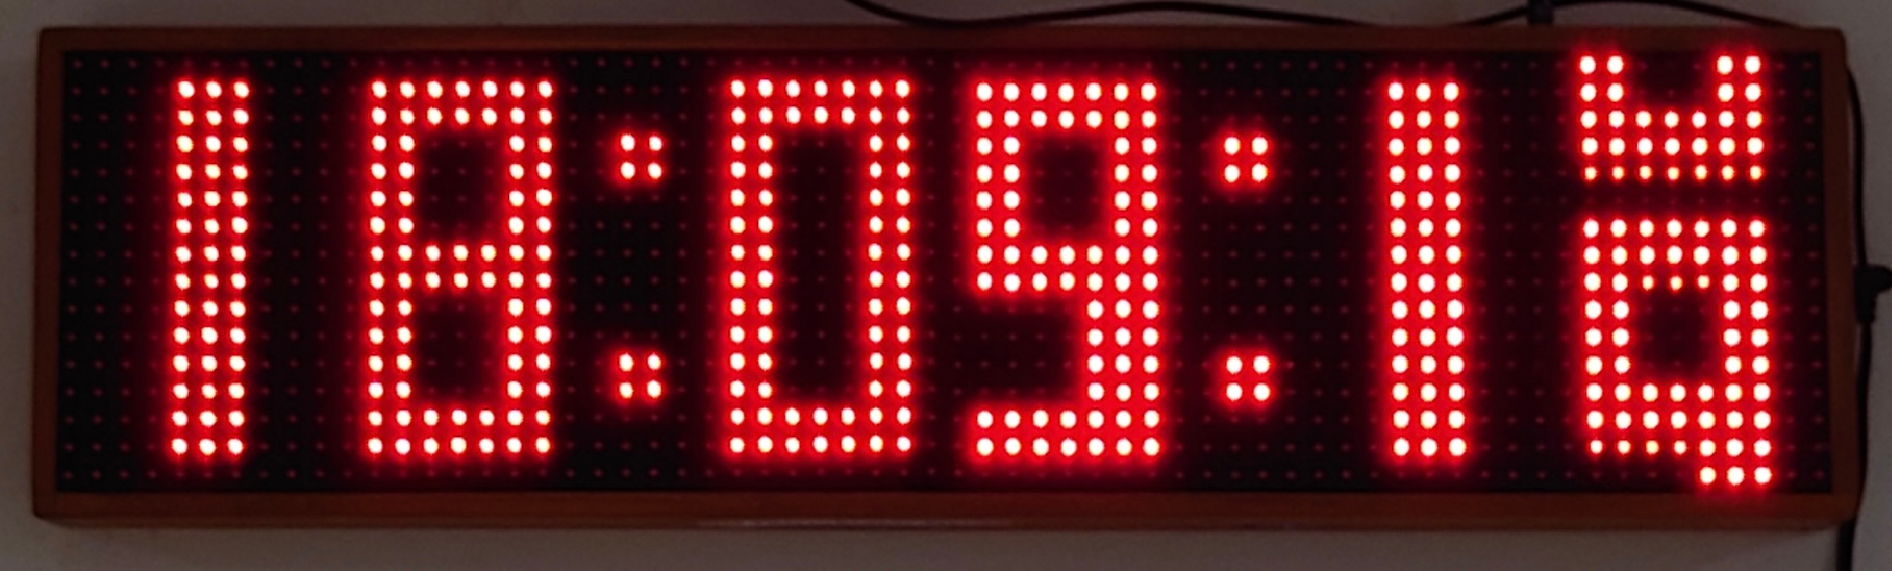
\includegraphics[width=\columnwidth]{figs/clock.pdf}
\par\vspace{1pt}
{\footnotesize (a) Clock}\par\medskip
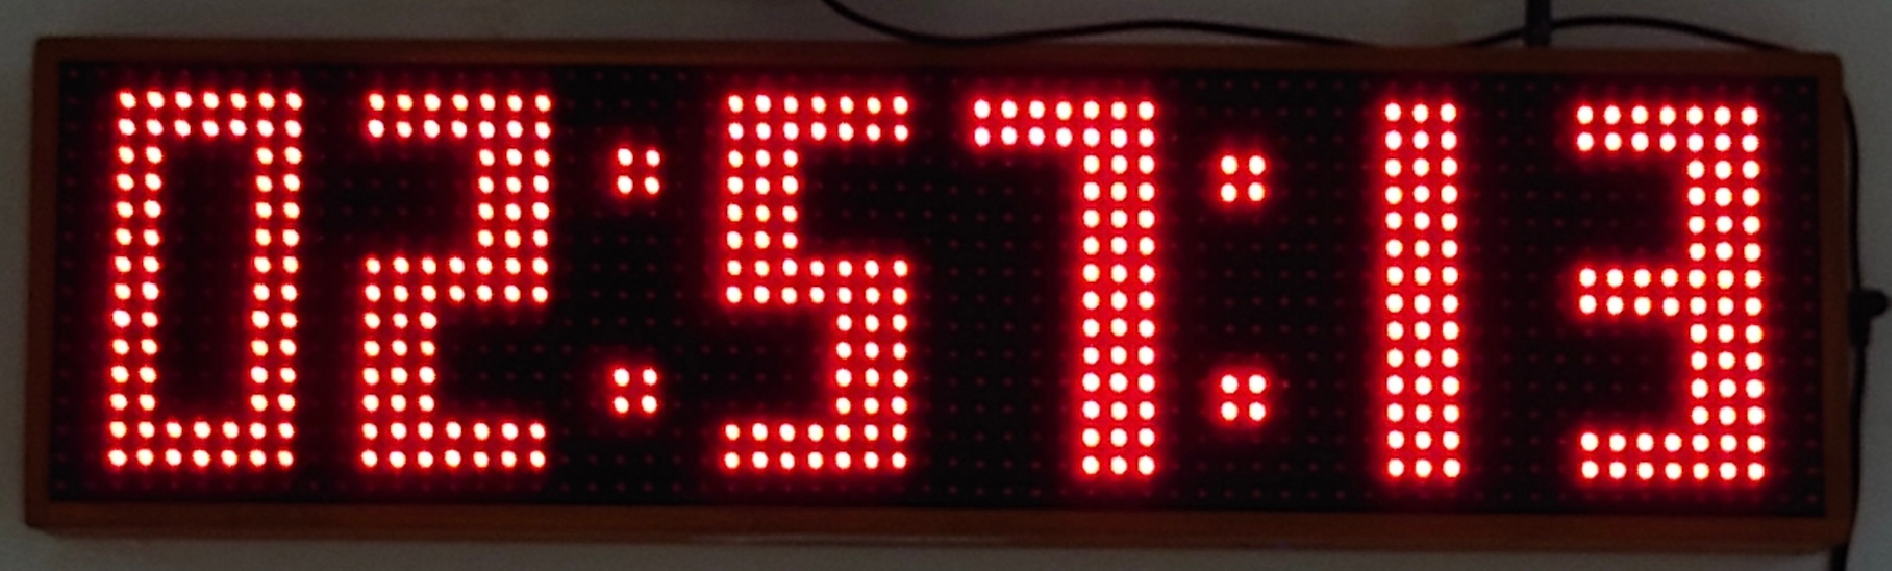
\includegraphics[width=\columnwidth]{figs/timer.pdf}
\par\vspace{1pt}
{\footnotesize (b) Countdown}\par\medskip
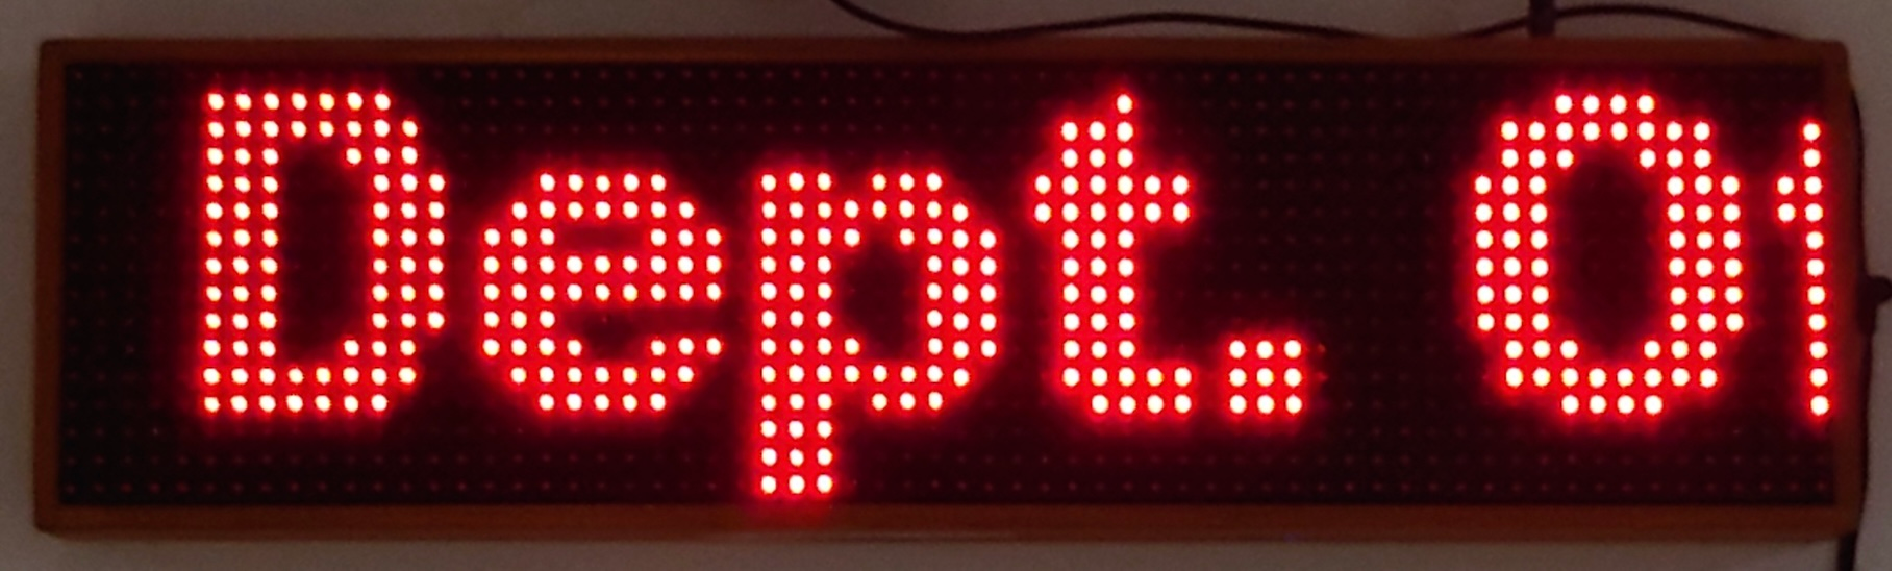
\includegraphics[width=\columnwidth]{figs/notice.pdf}
\par\vspace{1pt}
{\footnotesize (c) Scrolling notice}
\caption{An installed display operating in three modes.}
\label{fig:display}
\end{figure}

We deployed ten units at Shahjalal University of Science and Technology, Bangladesh (Fig.~\ref{fig:display}). Teachers and staff use the displays for timekeeping, announcements, important notices, and examination scheduling in spaces ranging from corridors and offices to classrooms and examination halls.